
\section{A theory of social systems}
The German sociologist Luhmann proposed, in his seminal work \citep{Luhmann94} a
new theory about how communications generate societies. Important to his
work is the underlying assumption that organisms act as closed loop systems
\citep{Wiener61,Glasersfeld1995} who pursue their own goals and are not able to observe
the internal states nor the inputs of other organisms \citep{vonFoerster60}.
A central assumption is that agents are continuously trying to reduce their own
perceived uncertainty of their environment (perceived complexity from the
agent's point of view). This is done by learning to anticipate events in the
environment. For example an agent can learn to use vision to prevent falling off
a cliff \citep{Verschure91}. In other words agents aim to turn
themselves from reactive into proactive closed loop systems.
In the social context this becomes more complex when learning agents try to
predict each other. Because agents cannot observe the internal states of the
other agents, the system becomes more unpredictable. Parsons called this the
“double contingency” problem \citep{Parsons77}:
Ego is trying to predict Alter, but Alter does the same.
In the case of two agents the double contingency problem might still
be treatable. However, when there are more than two agents the uncertainty
grows.
In order to reduce the uncertainty Luhmann proposed that social systems
have to create subsystems which specialize \citep{Luhmann94} in the sense that
they form sub-groups by executing only a subset of behaviours and/or agents
only perceive certain aspects of the environment and not all.
A fundamental condition for the formation of sub-systems is communication, 
which Luhmann uses in a broader sense compared to the concept of language.
There have been attempts to model aspects of social system theory, which 
will be discussed in Section \ref{Chapter1:SocialSystemTheory}.
The first model which incorporated Luhmann's principles belongs to 
\citet{SocialOrderScalability} which used 
double contingency as the origins of social order. 
Luhmann's communication is the distinction between information, transmission
and understanding, which is required if the agents operate as autonomous close
loop systems. Also agents show meaningful motivated behaviour towards
others, according to goals and a shared symbolic system, as proposed in Parson's
models \citep{Parsons51,Parsons77}.
The next section describes a very important modelling approach particularly suited
for social systems.

\section{Modelling approach ABM}
Agent Based Modelling is a powerful tool where the researcher has to simulate a complex
system like a social system \citep{WMacyWiller2002:SocialABM}.
A social system is composed of an agent or entities which interact with each
other and the environment.
Every entity is described by a set of behaviours or rules which can be static
or dynamic.
The interaction can be at the action level or at the communication level.
Traditional approaches are based on logic of formal analysis) or on
mathematical models of differential and partial equations.
The formal analysis - also known as model checking- can be used to verify if a
property of the system is valid or not, without the need of applying statistic
on a large set of simulations.
Model checking, if properly used, can be a powerful tool for the analysis of
social models and was also applied in parallel to the ABM model (see the Conclusion
for a more detailed explanation).
The approach with differential equations is only feasible when the model can 
be described analytically and has been very effective to model the dynamic of biological
populations like the well famous Lotke Volterra equations \citep{LotkeVolterra1931:PredatorPrey} that describes the
 evolution of predator-prey populations 
The differential equations are formulated over the general behaviour of the system
 and do not take into account individual interactions that are the main 
purpose of research in this study.
The model becomes even more complicated when each agent has an adaptive
behaviour which changes in time with the others: this means that every
agent is initially identical but as time progresses and interactions are
performed, dissimilarities emerge and thus a new collective behaviour emerges.

The ABM approach was chosen not only for the with the aim of implementing the simulated system
 in a real robotic hardware.
Thanks to the ABM approach an agent that has been embodied in a software simulation,
 can be easily embodied in a real robot.
The advantage is then not only the time required to realise such a system,
but also the expected behaviour of the robot that will match the simulated behaviour.
There are a numbers of potential software frameworks that can be used to
implement ABM systems and these will be discussed in Section
\ref{Chapter3:ABMcomplex}.

\section{Objectives and Motivation of the thesis}
The motivation behind this research is the implementation of Luhmann's
principles for the generation of artificial social systems.
Luhmann formulated a theory that has produced a considerable
impact in sociology but there have only been a few attempts to validate
the theory experimentally.
This is what has motivated this thesis in terms of experiment setup and
validation of the model.
The validation of the model, even to a limited extent of sub-properties of the
original theory, is an important step for the understanding of not only
artificial societies but also of human like processes.
It could help in the future to predict the effect of a policy (normative order)
on a human population or to build robots which are able to cooperate and
interact socially between themselves and human operators.
This is why the modelling approach used in this work is based on biological
inspired behaviour which captures the natural behaviour of simple animals and
can easily be transferred into an embodied robotic system.
A conceptual diagram of the thesis and of the work is shown in 
Figure \ref{fig:overview-1} and Figure \ref{fig:overview-2}.

\begin{figure}[htbp]
\begin{center}
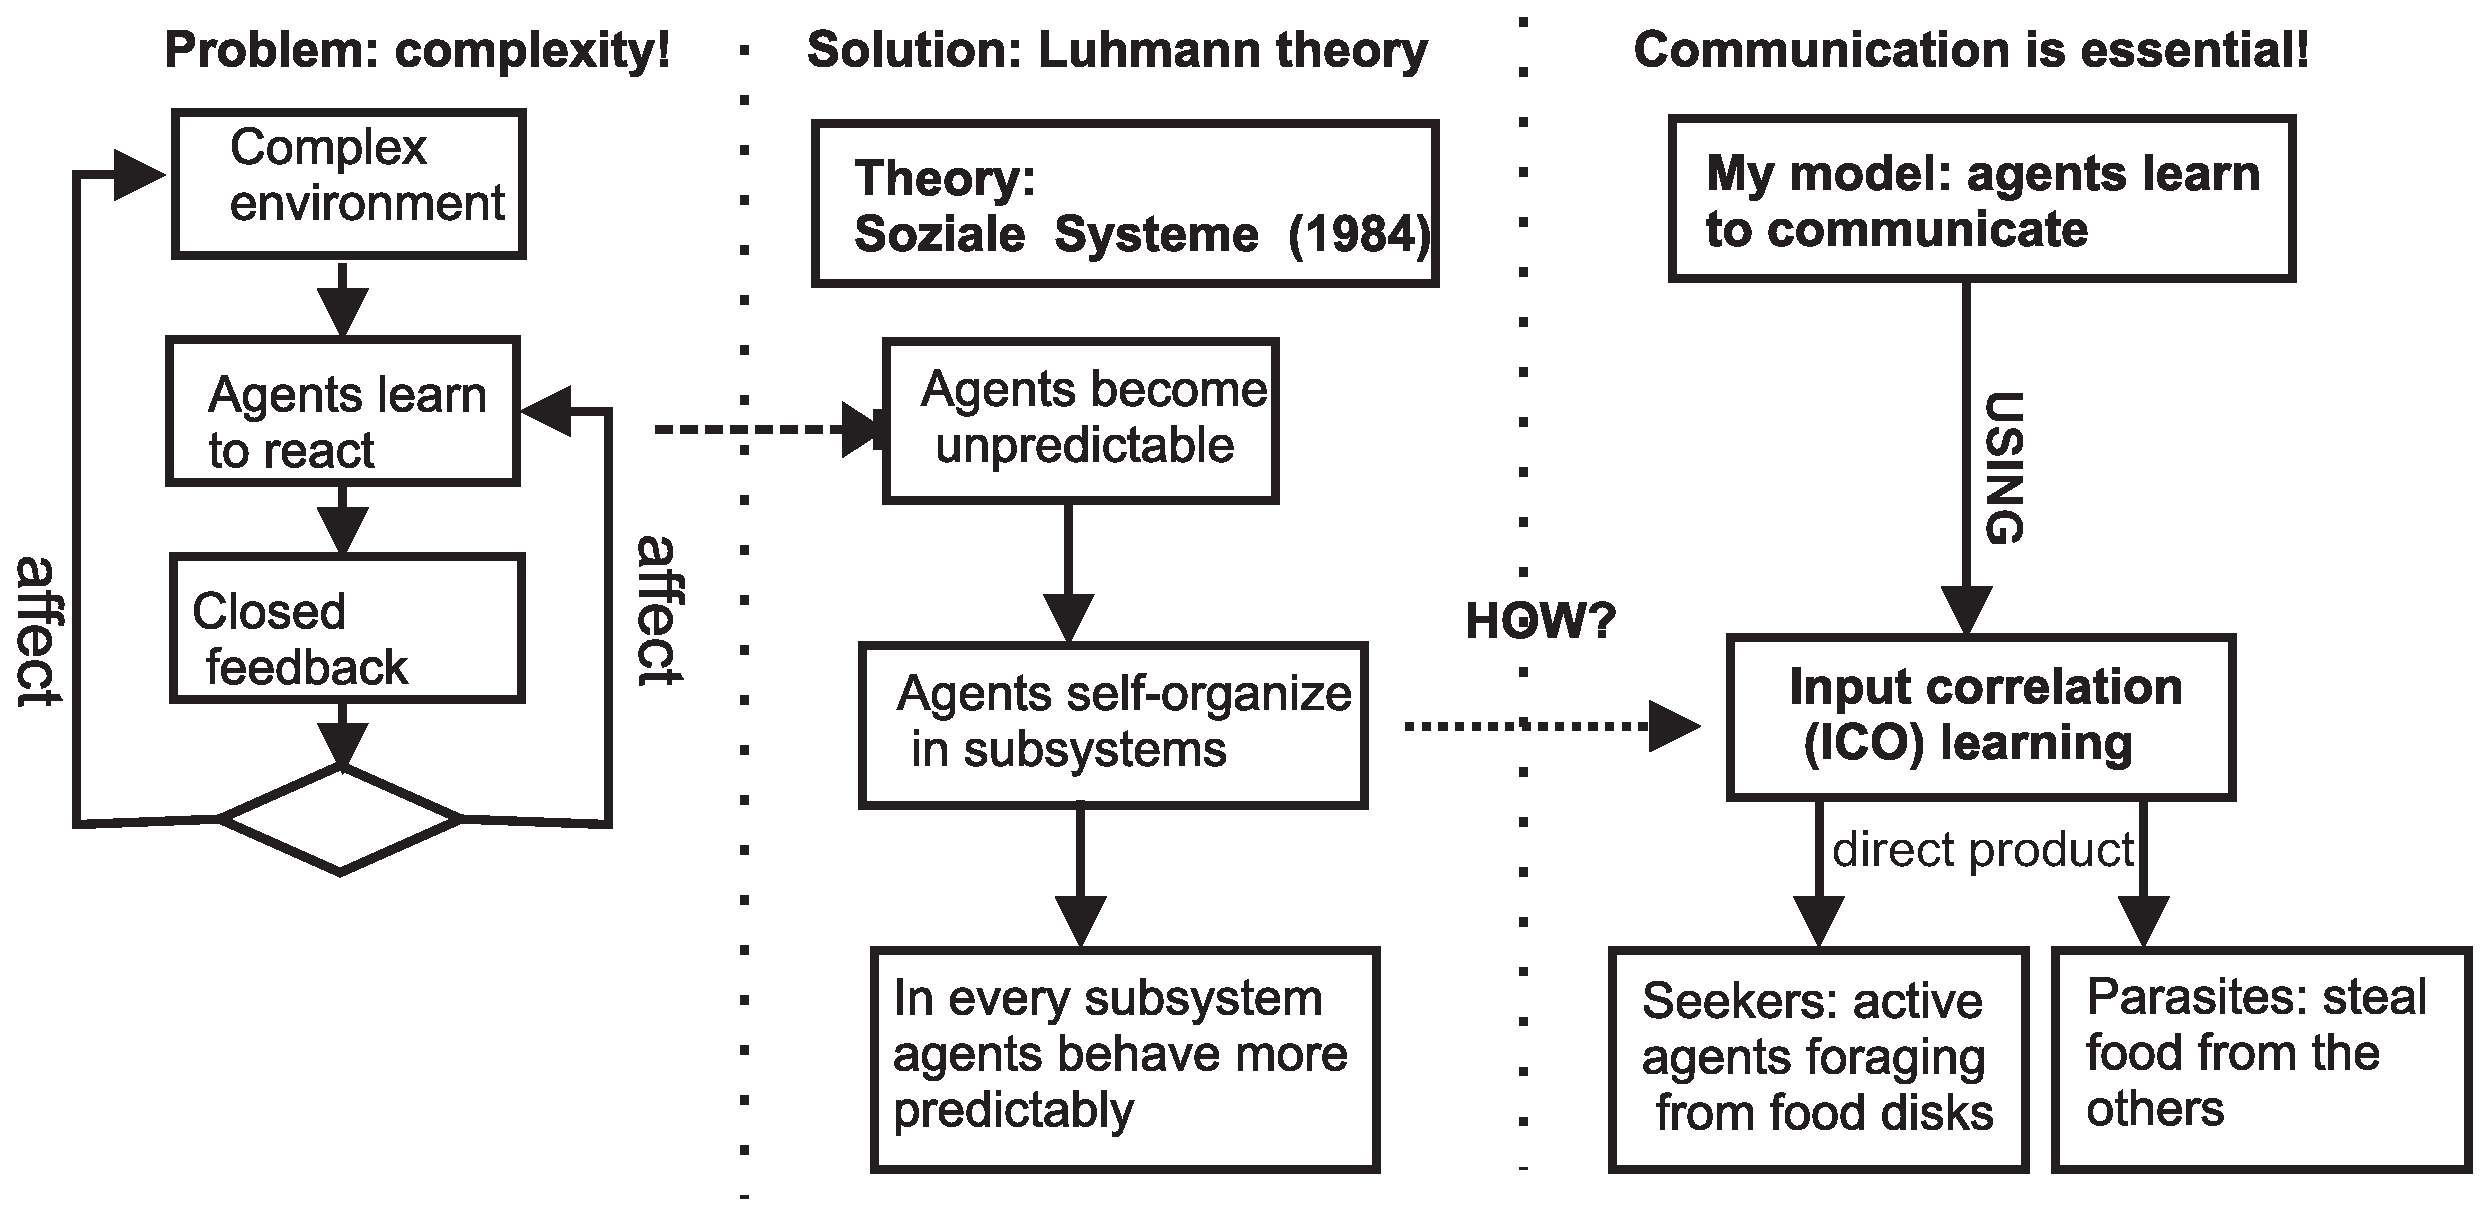
\includegraphics[width=1.0 \textwidth]{overview-1.eps}
\end{center}
\small{
\caption[Thesis research aim system]{Thesis objective at the system level \label{fig:overview-1}}}
\end{figure}

\begin{figure}[htbp]
\begin{center}
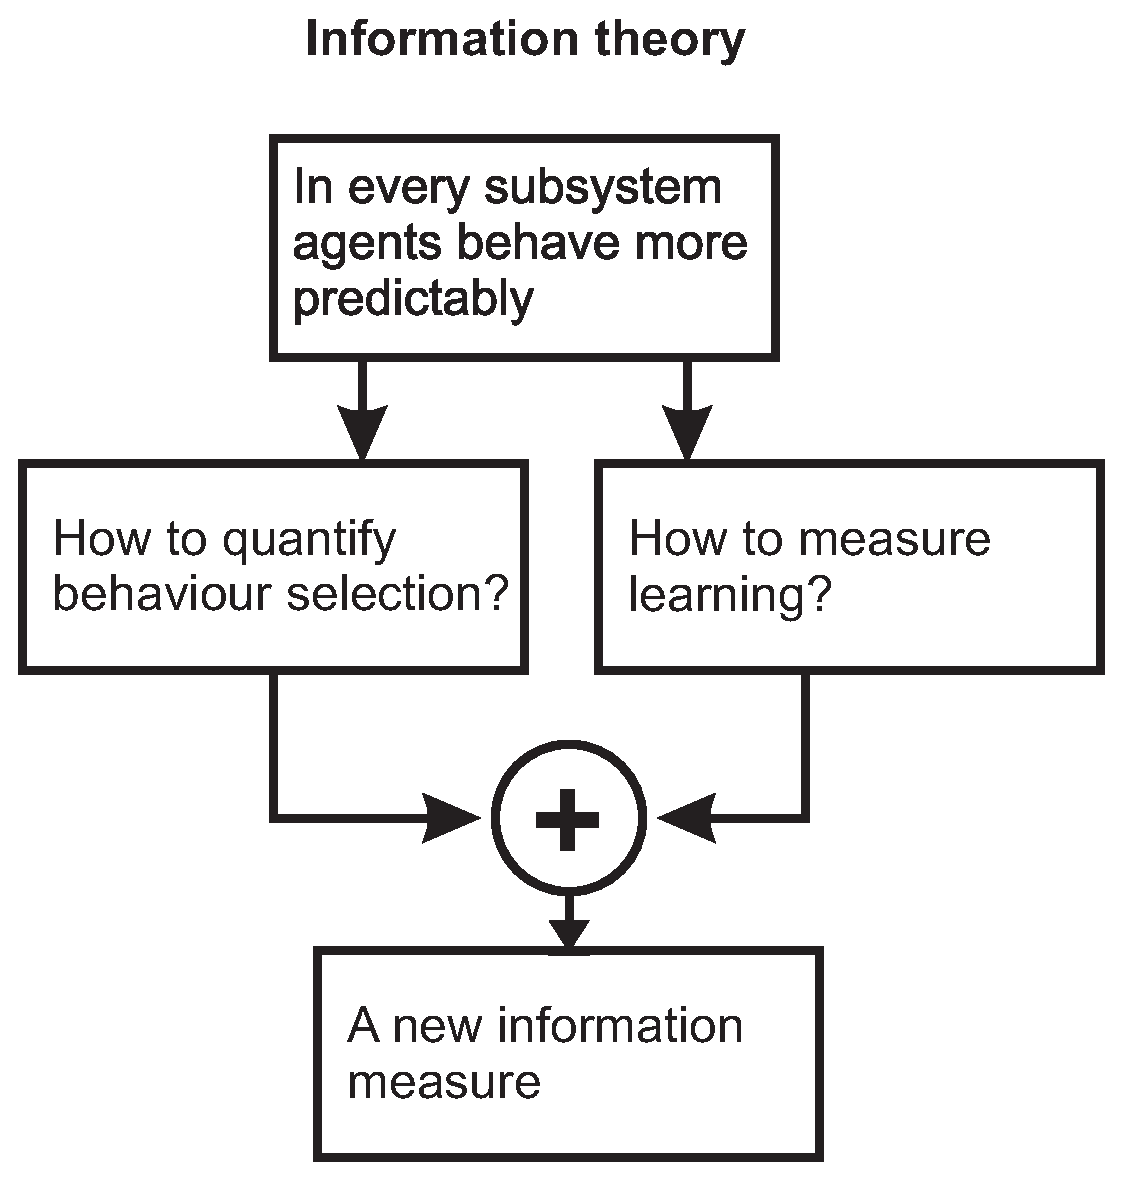
\includegraphics[width=0.5 \textwidth]{overview-2.eps}
\end{center}
\small{
\caption[Thesis research aim individual]{Thesis objective at the individual level \label{fig:overview-2}}}
\end{figure}

\section{Aim}

The aim of the thesis is to investigate the formation of sub-systems at a
system level as summarised in Figure \ref{fig:overview-1} and to
investigate the behaviour at an individual level as summarised in Figure \ref{fig:overview-2}.

The objectives of the thesis can be then summarised:
\begin{itemize}
\item implement a social system based on the Luhmann's hypothesis
\item verify the self-organising property (autopoiesis principle) of the system
\item measure the self-organising property of the system
\item quantify the self-organising property at the individual level with an
information theoretic approach
\item apply the same approach to different models
\end{itemize}

\section{Outline of thesis}
The thesis is divided into the following chapters:
\begin{itemize}
 \item this Chapter is a general introduction to this thesis
and a quick review of the existing literature.
 \item Chapter \ref{Chapter:Review} is a detailed review of literature closely related to this thesis.
 \item Chapter \ref{Chapter:Work} contains the main research and results
carried out by the author during his Ph.D.
 \item Chapter \ref{Conclusion} contains a summary of the results, a critical
comparison with the existing literature, a description of future work
and possible or existing industrial applications.
\end{itemize}

In Chapter \ref{Chapter:Work}, each Section was written to be a self-contained
module structured in the familiar order: Introduction, Methods, Results, and Discussion.
To avoid too much fragmentation a simple notation was used, for example in 
Chapter \ref{Chapter:Work}, Section \ref{Chapter7:Q learning application} 
is divided as follows:
\begin{itemize}
 \item Introduction: the application of information flow to Q-learning
 \item Methods: reinforcement learning
 \item Methods: Q-Learning algorithm
 \item Methods: Q-Learning connectionist
 \item Methods: The robot and the task
 \item Results: avoidance case
 \item Discussion
\end{itemize}
Each entry is then prefixed with the corresponding order.
All the sections are ordered in a logical manner, which does not correspond directly
to the chronological order of the research.
This happened for example with the Predictive Performance measure, which was
developed for a retinal robot and only after was applied to the data generated for
 the social system.
I have chosen a logical order so that the reader will be introduced gradually
to the topics.


